\tikzsetexternalprefix{tikz/}	% set subfolder
\tikzsetnextfilename{Train_evolution}

%\newcommand{\righttriangles}[1]{
%    \pgfplotstableread[col sep=tab, header=true]{#1}{\table}
%    \pgfplotstablegetcolsof{#1}
%    \pgfmathtruncatemacro\numberofcols{\pgfplotsretval - 1}
%    \pgfplotsinvokeforeach{1,...,\numberofcols}{
%        \pgfplotstablegetcolumnnamebyindex{##1}\of{\table}\to{\colname}
%        \addplot [name path=down##1, semithick, color##1, mark=*, mark size=1, mark options={solid}]%
%        		table [x index= 0, y index=##1] {#1};
%        \addlegendentryexpanded{ \SI{\colname}{\mW} }
%    }
%}

%\newcommand{\lefttriangles}[1]{
%    \pgfplotstableread[col sep=tab, header=true]{#1}{\table}
%    \pgfplotstablegetcolsof{#1}
%    \pgfmathtruncatemacro\numberofcols{\pgfplotsretval - 1}
%    \pgfplotsinvokeforeach{1,...,\numberofcols}{
%        \pgfplotstablegetcolumnnamebyindex{##1}\of{\table}\to{\colname}
%        \addplot [name path=up##1, semithick, color##1, mark=*, mark size=1, mark options={solid}]%
%        		table [x index= 0, y index=##1] {#1};
%    }
%}

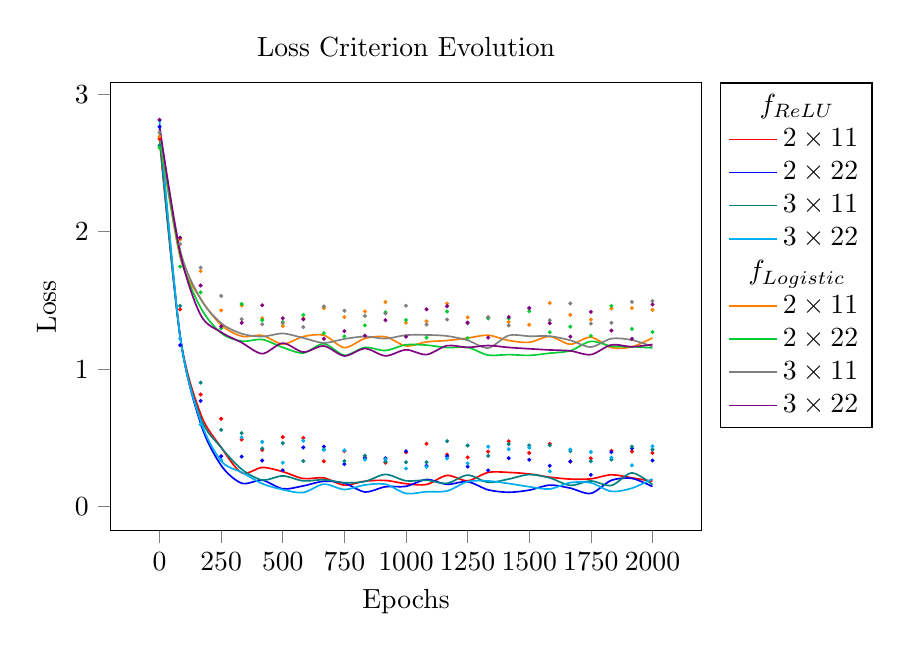
\begin{tikzpicture}[baseline]

%	\definecolor{color1}{rgb}{0.12156862745098,0.466666666666667,0.705882352941177}
%	\definecolor{color2}{rgb}{1,0.498039215686275,0.0549019607843137}
%	\definecolor{color3}{rgb}{0.172549019607843,0.627450980392157,0.172549019607843}
%	\definecolor{color4}{rgb}{0.83921568627451,0.152941176470588,0.156862745098039}
%	\definecolor{color5}{rgb}{0.580392156862745,0.403921568627451,0.741176470588235}
%	\definecolor{color6}{rgb}{0.549019607843137,0.337254901960784,0.294117647058824}
%	\definecolor{color7}{rgb}{0.890196078431372,0.466666666666667,0.76078431372549}
%	\definecolor{color8}{rgb}{0.45,0.45,0.45}
%	\definecolor{color9}{rgb}{0.25,0.25,0.99}
	
	\begin{axis}[
			title={Loss Criterion Evolution},
			xlabel={Epochs},
			ylabel={Loss},
			tick align=outside,
			tick pos=left,
			width=\textwidth*0.75,
			height=207pt,
			legend pos = outer north east,
%			cycle list name=color list,
			/pgf/number format/1000 sep=,
%			xmin=-199, xmax=2199,
			xtick distance=250,
			domain=0:2000,
			train/.style={
				smooth,
				semithick,
			},
			valid/.style={
				only marks,
				mark=*,
				mark options={scale=0.25},
				forget plot,
			},
		]
		\addlegendentry{\hspace{-.6cm}$f_{ReLU}$};
		\addlegendimage{empty legend};

		\addplot [red, train] {0.2+2.5*exp(-0.01*x)+0.05*rand};
		\addlegendentry{$2\times 11$}
		\addplot [red, valid] {0.4+2.3*exp(-0.01*x)+0.1*rand};
		
		\addplot [blue, train] {0.15+2.6*exp(-0.011*x)+0.06*rand};
		\addlegendentry{$2\times 22$}
		\addplot [blue, valid] {0.35+2.35*exp(-0.012*x)+0.13*rand};

		\addplot [teal, train] {0.2+2.5*exp(-0.01*x)+0.05*rand};
		\addlegendentry{$3\times 11$}
		\addplot [teal, valid] {0.4+2.3*exp(-0.01*x)+0.1*rand};
		
		\addplot [cyan, train] {0.15+2.6*exp(-0.011*x)+0.06*rand};
		\addlegendentry{$3\times 22$}
		\addplot [cyan, valid] {0.35+2.35*exp(-0.012*x)+0.13*rand};
%		red,blue,black,yellow,brown,teal,orange,violet,cyan,green!70!black,magenta,gray
		
		\addlegendentry{\hspace{-.6cm}$f_{Logistic}$}
		\addlegendimage{empty legend};
		
		\addplot [orange, train] {1.2+1.5*exp(-0.01*x)+0.05*rand};
		\addlegendentry{$2\times 11$}
		\addplot [orange, valid] {1.4+1.3*exp(-0.01*x)+0.1*rand};
		
		\addplot [blue!20!green, train] {1.15+1.6*exp(-0.011*x)+0.06*rand};
		\addlegendentry{$2\times 22$}
		\addplot [blue!20!green, valid] {1.35+1.35*exp(-0.012*x)+0.13*rand};	
		
		\addplot [gray, train] {1.2+1.5*exp(-0.01*x)+0.05*rand};
		\addlegendentry{$3\times 11$}
		\addplot [gray, valid] {1.4+1.3*exp(-0.01*x)+0.1*rand};
		
		\addplot [violet, train] {1.15+1.6*exp(-0.011*x)+0.06*rand};
		\addlegendentry{$3\times 22$}
		\addplot [violet, valid] {1.35+1.35*exp(-0.012*x)+0.13*rand};
		
	\end{axis}
\end{tikzpicture}